\section{Funktionsmodellierung}
\label{fm}
Nachdem die Regressionsanalyse in \vref{dmmethoden} als Data-Mining-Methode für diese Arbeit festgelegt wurde, wird der Leser im folgenden Kapitel mit den grundlegenden Bestandteilen der Funktionsmodellierung mit Hilfe der \gls{regression} vertraut gemacht (siehe \vref{ra}). Dazu werden die unterschiedlichen Modelle der Regression vorgestellt und in Bezug auf die vorliegende Problemstellung bewertet. Anschließend wird in \vref{matlab} das Software-Tool \gls{matlab} in Hinblick auf die Lösung und graphische Darstellungen von mathematischen Problemen vorgestellt. Die dafür bereitgestellten Funktionalitäten der Regressionanalyse werden innerhalb der späteren Umsetzung angewendet.


\subsection{Regressionsanalyse}
\label{ra}
\subsubsection{Allgemein}
Die \gls{regression} (lat. \textit{regredi} für umkehren, zurückkehren) beinhaltet im Allgemeinen die Analyse einer abhängigen Variablen von einer oder mehreren unabhängigen Variablen.\seFootcite{Vgl.}{S. 5}{Studenmund.2014} Dabei drücken die unabhängigen Variablen die abhängige Variable mittels einer \textit{Regressionsgleichung} aus.\seFootcite{Vgl.}{S. 475}{Fahrmeir.2007} Die in der mathematischen Gleichung beinhaltenden Parameter (auch \textit{Regressoren} genannt) müssen so gewählt und justiert werden, dass eine möglichst genaues \textit{Fitting} (\textit{z.dt. Anpassung}) der resultierenden Funktion an die vorhandenen Daten erzielt wird.\seFootcite{Vgl.}{S. 68}{Gunther.2014}\seFootcite{Vgl.}{S. 1-2}{Schimek.2000} Diese rein datenbasierte mathematische Beschreibung hat ihren Ursprung in einer Studie von Francis Galton\footnote{britischer Naturforscher im 19. Jahrhundert - prägte erstmals den Begriff der \textit{\gls{regression}}.}, in der die Körpergröße von Kindern im Verhältnis zu derer ihrer Eltern analysiert wurde.\seFootcite{Vgl.}{S. 68}{Gunther.2014} Anhand der vorliegenden Problemstellung dieser Arbeit, lässt sich das Vorgehen der Regressionsanalyse beispielhaft demonstrieren:

Es wird versucht, die Abhängigkeit der Wahrscheinlichkeit eines Torerfolges (\textit{=abhängige Variable}), von Einflussfaktoren, wie der Distanz oder des Winkels zum Tor bzw. der Koordinaten des Schusses (\textit{=unabhängige Variablen}), mit Hilfe einer Funktion (\textit{=Regressionsgleichung}) zu ermitteln. 

Anhand der \textit{linearen Regression} sollen die grundlegenden Bestandteile aller Regressionsmodelle erläutert werden. Um eine Punktewolke (die beobachteten Daten) durch eine Funktion $\hat{f}$ zu approximieren, bedient man sich der quadratischen Abstände der Datenpunkte zur Funktion und versucht diese durch die \gls{mdkq} zu minimieren.\seFootcite{Vgl.}{S. 44}{Hastie.2016} Die lineare Regressionsfunktion liegt dabei in der Form 

\begin{equation}
	\hat{f}(x) = \hat{\alpha} \cdot x + \hat{\beta}
	\label{lrf}
\end{equation}

vor.\seFootcite{Vgl.}{S. 476}{Fahrmeir.2007} Wie in \vref{lr} exemplarisch dargestellt ist, werden die Abstände zwischen den beobachteten Datenpunkten (orangefarbene Kreise) und der Funktion ($y_i -  \hat{y}(x_i) \rightarrow i= 1,...,m$) summiert, woraus sich die \textit{Summe der Fehlerquadrate} (=\gls{rss}) ergibt:\seFootcite{Vgl.}{S. 37}{Studenmund.2014}

\begin{equation}
	RSS = \sum\limits_{i=1}^n (y_i - \hat{y}(x_i))^2
\end{equation}

Durch die Berechnung der \gls{rss} wird die Distanz zwischen den Daten und dem Modell berechnet. Um eine möglichst genaue Abbildung der Daten durch das Modell gewährleisten zu können, müssen die Parameter $\hat{\alpha}$ und $\hat{\beta}$ so gewählt werden, dass die Summe der Fehlerquadrate minimal ist.\seFootcite{Vgl.}{S. 69}{Gunther.2014} Es gilt:

\begin{equation}
	\min\limits_{a,b\in\mathbb{R}} RSS
\end{equation}

Das mathematische Vorgehen für die Ermittlung des Minimums einer Funktion mit mehreren Variablen -- partielle Ableitung von RSS($\hat{\alpha},\hat{\beta}$) -- wird verwendet, um die Parameter der Regressionsfunktion zu ermitteln:\seFootcite{Vgl.}{S. 39}{Studenmund.2014}

\begin{equation}
	\hat{\alpha} = \frac{\sum\limits_{i=1}^m x_i y_i - m \overline{x} \overline{y}}{\sum\limits_{i=1}^m x^2_i - m \overline{x}^2}
\end{equation}

\begin{equation}
	\hat{\beta} = \overline{y} - \hat{\alpha} \overline{x}^2
\end{equation}

Diese grundlegenden Bestandteile finden sich in allen Regressionsmodellen wieder, die in \vref{rm} kurz vorgestellt werden. 

%%%%%%%%%%%%%%%%%%%%%%%%%%%%%%%%%%%%%%%%%%%%%%%%%%

\subsubsection{Regressionsmodelle}\label{rm}
In der Praxis haben sich durch den allgemeinen Ansatz der \gls{regression} eine Vielzahl von Modellen etabliert, die je nach Anwendungsfall ihre Verwendungen finden:


\begin{itemize}

%%%%%%%%%%%%% LINEARE REGRESSION %%%%%%%%%%%%%%%%%%

\item \textbf{Lineare Regression}
\\ Am bekanntesten ist die lineare Regression, die auch oft als \glqq Ausgleichsgerade\grqq~bezeichnet wird und zur Prognose einer unabhängigen Größe $y$, in Abhängigkeit \textit{einer} bekannten Größe $x$, angewendet wird.\seFootcite{Vgl.}{S. 475}{Fahrmeir.2007} Eine Funktion $\hat{f}(x)$ wie \vref{lrf} ist von ihren Regressoren $\alpha$ und $\beta$ \textit{linear} abhängig und heißt deshalb \textit{lineare Regressionsfunktion}.\seFootcite{Vgl.}{S. 68}{Gunther.2014}\enlargethispage{\baselineskip} In \vref{lr} ist eine solche Funktion beispielhaft dargestellt.
\begin{figure}[H]
\centering
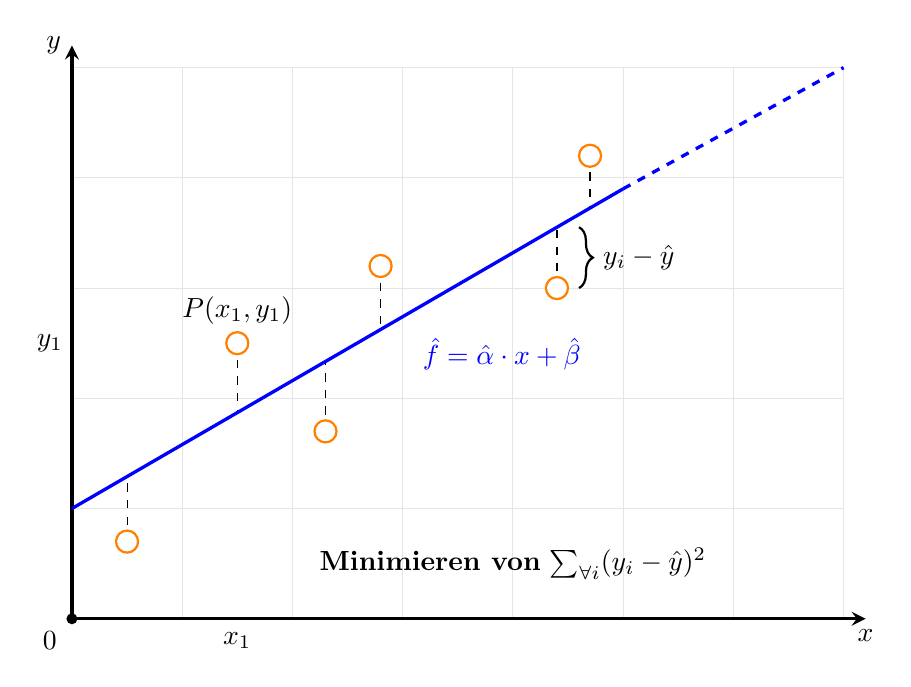
\begin{tikzpicture}[
	scale=1.4,
	axis/.style={
		-stealth,
		very thick
	},
	f/.style={
		very thick,
		blue
	}
]

% Gitter
\draw[gray!20] (0,0) grid (7,5);

% Achsen
\draw[axis] (0,0) -- (7.2,0) node[below]{$\boldsymbol{x}$};
\draw[axis] (0,0) -- (0,5.2) node[left]{$\boldsymbol{y}$};
\fill[black] (0,0) circle[radius=0.05];
\node at(-0.2,-0.2){$\boldsymbol{0}$};

% Punkte
\foreach \x/\y in {0.5/0.7,1.5/2.5,2.3/1.7,2.8/3.2,4.4/3,4.7/4.2}{
	\draw[dashed,domain=\x:\x,variable=\z] (\x,\y) -- plot ({\z},{2.9/5*\z+1});
	\draw[orange,thick,fill=white] (\x,\y) circle[radius=0.1cm];
}

% Funktion
\draw[f] (0,1) -- (5,3.9);
\node[blue] at(3.9,2.4){$\boldsymbol{\hat{f} = \hat{\alpha} \cdot x + \hat{\beta}}$};
\draw[f,dashed] (5,3.9) -- (7,5);

% Geschweifte Klammer
\draw[
	thick,
	black,
	decorate,
	decoration = {
		brace,
		amplitude = 5pt
	}
] (4.6,3.552) -- (4.6,3)
	node[
		midway,
		right,
		xshift = 5pt
] {$\boldsymbol{y_i -  \hat{y}}$};


\node at(-0.2,2.5){$y_1$};
\node at(1.5,-0.2){$x_1$};
\node at(1.5,2.8){$\boldsymbol{P(x_1,y_1)}$};
\node at(4.0,0.5){\textbf{Minimieren von} $\boldsymbol{\sum_{\forall i}(y_i - \hat{y})^2}$};

\end{tikzpicture}
\caption[Graphische Darstellung der linearen Regression]{Graphische Darstellung der linearen Regression\protect\footnotemark}
\label{lr}
\end{figure}
\footnotetext{Abbildung in Anlehnung an \textit{Backhaus} et al., Multivariate Analysemethoden, 2016, S. 71.}


%%%%%%%%%%%%% NICHT LINEARE REGRESSION %%%%%%%%%%%%%%%%%%

\item \textbf{Nichtlineare Regression}

In vielen realen Anwendungen kann die Regressionsfunktion nicht durch die Linearkombination der Regressionskoeffizienten berechnet werden, da diese in \textit{linearer} Weise von den Regressoren abhängt. Allgemein lässt sich dieses Modell mit $\boldsymbol{x} = (x_1,...,x_n)$ und $\boldsymbol{a} = (a_1,...,x_s)$ wie folgt ausdrücken:\seFootcite{Vgl.}{S. 85}{Gunther.2014}

\begin{equation}
	\hat{f}(\boldsymbol{x}) = f(\boldsymbol{x},\boldsymbol{a})
\end{equation}

In \vref{nlr} liegen die Daten in einem oszillierenden, sinusförmigen Muster vor und können folglich mit der allgemeinen Sinusfunktion beschrieben werden ($\hat{f} = \alpha_0 \cdot \sin(\alpha_1 \cdot (x-\alpha_2))$). Bei dieser nichtlinearen Regressionsfunktionen können die Regressoren dazu verwendet werden, die Funktion möglichst genau an die Daten anzupassen, wobei $\alpha_0$ die Amplitude bestimmt, $\alpha_1$ die Periodenlänge und $\alpha_2$ die Sinus-Funktion entlang der $x$-Achse verschiebt.\seFootcite{Vgl.}{S. 85-86}{Gunther.2014} Auch hier lassen sich mit Hilfe des Standardmodells, der Minimierung der kleinsten Quadrate (\gls{mdkq}), die Parameter bestimmen.\seFootcite{Vgl.}{S. 509}{Fahrmeir.2007}

\begin{figure}[H]
\centering
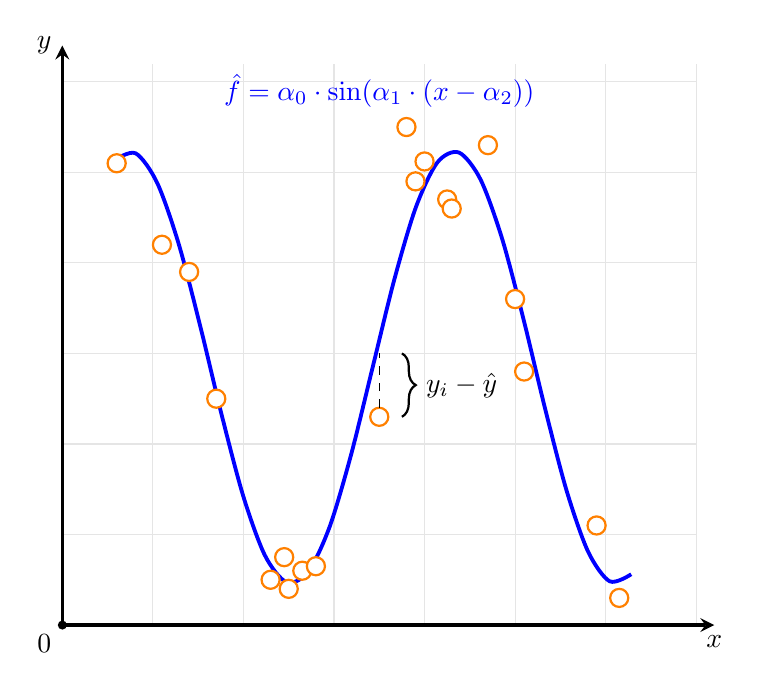
\begin{tikzpicture}[
	scale=1.15,
	axis/.style={
		-stealth,
		very thick
	}
]
% Gitter
\draw[gray!20] (0,0) grid (7,6.2);

% Achsen
\draw[axis] (0,0) -- (0,6.4) node[left]{$\boldsymbol{y}$};
\draw[axis] (0,0) -- (7.2,0) node[below]{$\boldsymbol{x}$};
\fill[black] (0,0) circle[radius=0.05];
\node at(-0.2,-0.2){$\boldsymbol{0}$};
    
    \begin{axis}[tick = none, axis lines=none]
    \addplot[smooth, color=blue, very thick] {sin(deg(x))}; 
    \end{axis}
    
    \node[blue] at(3.5,5.9){$\boldsymbol{\hat{f} = \alpha_0 \cdot \sin(\alpha_1 \cdot (x-\alpha_2))}$};
    
    \draw[orange,thick,fill=white] (1.1,4.2) circle[radius=0.1cm];
    \draw[orange,thick,fill=white] (0.6,5.1) circle[radius=0.1cm];
    \draw[orange,thick,fill=white] (1.4,3.9) circle[radius=0.1cm];
    \draw[orange,thick,fill=white] (1.7,2.5) circle[radius=0.1cm];
     \draw[orange,thick,fill=white] (2.3,0.5) circle[radius=0.1cm];
    \draw[orange,thick,fill=white] (2.45,0.75) circle[radius=0.1cm];
    \draw[orange,thick,fill=white] (2.65,0.6) circle[radius=0.1cm];
    \draw[orange,thick,fill=white] (2.8,0.65) circle[radius=0.1cm];
     \draw[orange,thick,fill=white] (2.5,0.4) circle[radius=0.1cm];
     
    \draw[orange,thick,fill=white] (4.25,4.7) circle[radius=0.1cm];
    \draw[orange,thick,fill=white] (4,5.12) circle[radius=0.1cm];
    \draw[orange,thick,fill=white] (4.7,5.3) circle[radius=0.1cm];
       \draw[orange,thick,fill=white] (3.8,5.5) circle[radius=0.1cm];
    \draw[orange,thick,fill=white] (4.3,4.6) circle[radius=0.1cm];
    \draw[orange,thick,fill=white] (3.9,4.9) circle[radius=0.1cm];
    
      \draw[orange,thick,fill=white] (5.1,2.8) circle[radius=0.1cm];
    \draw[orange,thick,fill=white] (5,3.6) circle[radius=0.1cm];
    \draw[orange,thick,fill=white] (5.9,1.1) circle[radius=0.1cm];
    \draw[orange,thick,fill=white] (6.15,0.3) circle[radius=0.1cm];
    
  \draw[orange,thick,fill=white] (3.5,2.3) circle[radius=0.1cm]; 
  \draw[dashed] (3.5,2.4) -- (3.5,3);   
    
    % Geschweifte Klammer
\draw[
	thick,
	black,
	decorate,
	decoration = {
		brace,
		amplitude = 5pt
	}
] (3.75,3) -- (3.75,2.3)
	node[
		midway,
		right,
		xshift = 5pt
] {$\boldsymbol{y_i -  \hat{y}}$};
\end{tikzpicture}
\caption[Graphische Darstellung der nichtlinearen Regression]{Graphische Darstellung der nichtlinearen Regression\protect\footnotemark}
\label{nlr}
\end{figure}
\footnotetext{Abb. in Anlehnung an \textit{Günther}, Mathematische Modellbildung und Simulation, 2014, S. 86.}


%%%%%%%%%%%%% MULTIPLE REGRESSION %%%%%%%%%%%%%%%%%%

\item \textbf{Multiple Regression}\enlargethispage{\baselineskip} 
In den meisten technischen und wirtschaftlichen Anwendungsfällen ist die Zielvariable $y$ von mehr als einer unabhängigen Variablen abhängig. Dieser Fall kann durch die \textit{multiple} oder auch \textit{multivariate Regression} behandelt werden, wobei sich diese Regressionsfunktion mit den unabhängigen Variablen ($\boldsymbol{x} = (x_1,...,x_n)$) und beliebigen reellen Funktionen ($f_i$) im Allgemeinen wie folgt ausdrücken lässt:\seFootcite{Vgl.}{S. 41-42}{Studenmund.2014}

\begin{equation}
	\hat{f}(\boldsymbol{x}) = \alpha_0 + \alpha_1 f_1(\boldsymbol{x}) + \alpha_2 f_1(\boldsymbol{x}) + ... + \alpha_s f_s(\boldsymbol{x}) 
\end{equation}

Die Vorgehensweise zur Ermittlung der Parameter entspricht der linearen Regression -- auch hier wird die Methode zur Minimierung der kleinsten Quadrate (\gls{mdkq}) angewendet. Liegt beispielsweise eine Punktewolke wie in \vref{mr} vor, kann diese durch die Funktion

\begin{equation}
	\hat{f}(x_1,x_2) = \alpha_0 + \alpha_1 x_1 + \alpha_2 x_2
\end{equation}

beschrieben werden, wobei der Regressor $\alpha_0$ die Verschiebung der Fläche entlang der $y$-Achse, $\alpha_1$ die Steigung der Variable $x_1$ sowie $\alpha_2$ die Steigung von $x_2$ angibt. 

\begin{figure}[H]
\centering
\def\axislength{.2}
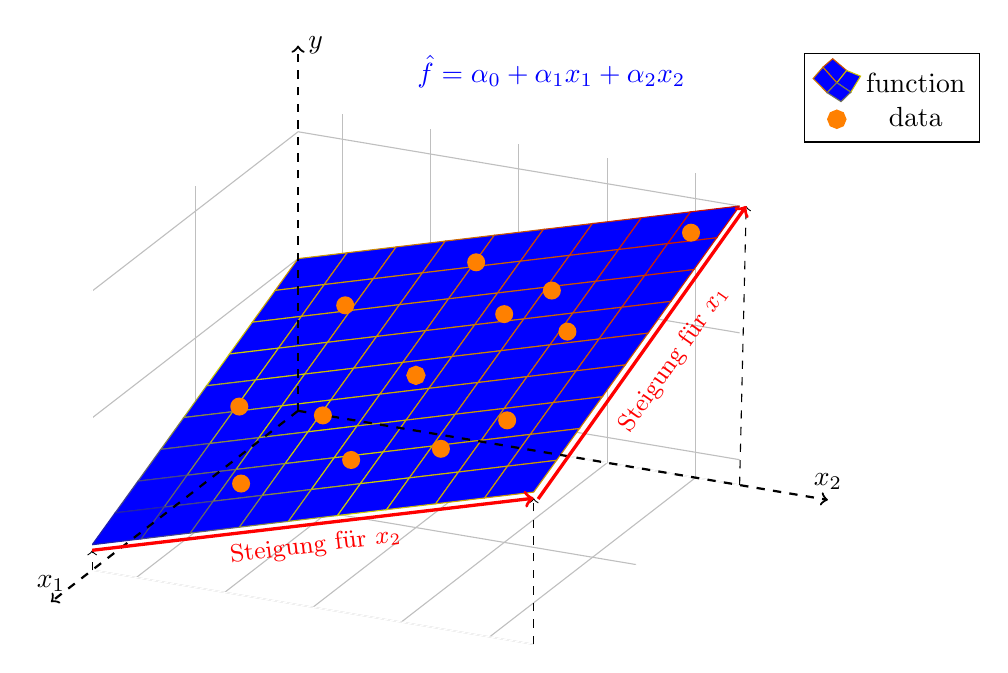
\begin{tikzpicture}
\pgfplotsset{
    axis line style={white},
  }
  \begin{axis}[scale=1.2,ticks=none, grid=major, legend style={at={(1.1,1.1)},anchor=north west} ]
    \coordinate (O) at (rel axis cs:0,1,0);
    \coordinate (x) at (rel axis cs:0,-\axislength,0);
    \coordinate (y) at (rel axis cs:1+\axislength,1,0);
    \coordinate (z) at (rel axis cs:0,1,1+\axislength);
    
    \coordinate (mx2b) at (rel axis cs:0,0,0.065);
    \coordinate (mx2e) at (rel axis cs:1,0,0.48);
     \coordinate (mx1e) at (rel axis cs:1.015,1,0.92);
    \coordinate (mx1b) at (rel axis cs:1.01,0,0.48);
    \coordinate (labelx1) at (rel axis cs:1,0.95,0.7);
    
    \coordinate (fst) at (rel axis cs:0,0,0);
    \coordinate (snd) at (rel axis cs:1,0,0);
    \coordinate (thd) at (rel axis cs:1,1,0);   
    
    \coordinate (f) at (rel axis cs:0.9,0.3,1.7);
    
    \coordinate (p1) at (rel axis cs:0.5,0.5,0.5);  
    \coordinate (p2) at (rel axis cs:0.23,0.23,0.22);
    \coordinate (p3) at (rel axis cs:0.71,0.71,0.72);
    
    \coordinate (p4) at (rel axis cs:0.2,0.8,0.5);  
    \coordinate (p5) at (rel axis cs:0.4,0.4,0.25);
    
    \coordinate (p6) at (rel axis cs:0.8,0.3,0.53);
    \coordinate (p7) at (rel axis cs:0.65,0.3,0.4);  
    
    \coordinate (p8) at (rel axis cs:0.45,0.9,0.65);
    
    \coordinate (p9) at (rel axis cs:0.35,0.37,0.4);
    \coordinate (p10) at (rel axis cs:0.1,0.5,0.3);  
   
    \coordinate (p11) at (rel axis cs:0.7,0.5,0.75);
    
    \coordinate (p12) at (rel axis cs:0.75,0.7,0.6);
    \coordinate (p13) at (rel axis cs:0.925,0.925,0.85);  
   
    \addplot3[surf, color=blue, samples=10] {x+y};
    \addlegendentry{function}
    \addplot3[mark=*,
			  only marks,
			  mark options={line width=0.1cm, color=orange,fill=orange}] coordinates{(0,0,0)};
    \addlegendentry{data}
  \end{axis}
  \draw[thick,dashed,->] (O) -- (x) node[above] {$\boldsymbol{x_1}$};
  \draw[thick,dashed,->] (O) -- (y) node[above] {$\boldsymbol{x_2}$};
  \draw[thick,dashed,->] (O) -- (z) node[right] {$\boldsymbol{y}$};
  
  \draw[dashed,->] (fst) -- (mx2b) node[above] {};
  \draw[dashed,->] (snd) -- (mx2e) node[right] {};
  \draw[dashed,->] (thd) -- (mx1e) node[right] {};
  
  \draw[red,very thick,->] (mx2b) -- (mx2e) node[rotate=7,below, midway] {\small Steigung für $x_2$};
  \draw[red,very thick,->] (mx1b) -- (mx1e) node[rotate=55,left] at (labelx1) {\small Steigung für $x_1$};
  
  \node[blue] at(f){$\boldsymbol{\hat{f} = \alpha_0 + \alpha_1 x_1 + \alpha_2 x_2}$};
  
  \draw[orange,thick,fill=orange] (p1) circle[radius=0.1cm];
  \draw[orange,thick,fill=orange] (p2) circle[radius=0.1cm];
  \draw[orange,thick,fill=orange] (p3) circle[radius=0.1cm];
  \draw[orange,thick,fill=orange] (p4) circle[radius=0.1cm];
  \draw[orange,thick,fill=orange] (p5) circle[radius=0.1cm];
  \draw[orange,thick,fill=orange] (p6) circle[radius=0.1cm];
  \draw[orange,thick,fill=orange] (p7) circle[radius=0.1cm];
  \draw[orange,thick,fill=orange] (p8) circle[radius=0.1cm];
  \draw[orange,thick,fill=orange] (p9) circle[radius=0.1cm];
  \draw[orange,thick,fill=orange] (p10) circle[radius=0.1cm];
  \draw[orange,thick,fill=orange] (p11) circle[radius=0.1cm];
  \draw[orange,thick,fill=orange] (p12) circle[radius=0.1cm];
  \draw[orange,thick,fill=orange] (p13) circle[radius=0.1cm];
  
\end{tikzpicture}
\caption[Graphische Darstellung der multiplen Regression]{Graphische Darstellung der multiplen Regression\protect\footnotemark}
\label{mr}
\end{figure}
\footnotetext{Eigene Darstellung.}

%%%%%%%%%%%%% NICHT PARAMETRISCHE REGRESSION %%%%%%%%%%%%%%%%%%

\item \textbf{Nichtparametrische Regression}
In vielen Anwendungen lässt sich nicht im Voraus vornherein eine Regressionsfunktion mit bestimmter Spezifizierung der Parameter vorhersagen. In den vorangehenden Beispielen -- linear wie nichtlinear -- wurde jeweils ein konkreter Ausdruck vorgegeben, um mittels Minimierung der kleinsten Quadrate (\gls{mdkq}) die Funktion an die Daten anzupassen. Betrachtet man \vref{pr}, so lässt sich erkennen, dass es hierzu keine passende mathematische Funktion geben kann.\seFootcite{Vgl.}{S. 91}{Gunther.2014} Die nichtparametrische Regression verfolgt das Ziel, die Funktion $\hat{f}$ möglichst genau zu schätzen. Etabliert haben sich hierbei Methoden wie \textit{Spline-Regressionen} und \textit{lokale Regressionsschätzer}, die jedoch aufgrund ihres numerischen Aufwands hier nicht detailliert beschrieben werden und selbst nur bei der Verwendung von statistischen Programmpaketen (vgl. MATLAB \vref{matlab}) Anwendungen finden.\seFootcite{Vgl.}{S. 510}{Fahrmeir.2007}

\begin{figure}[H]
\centering
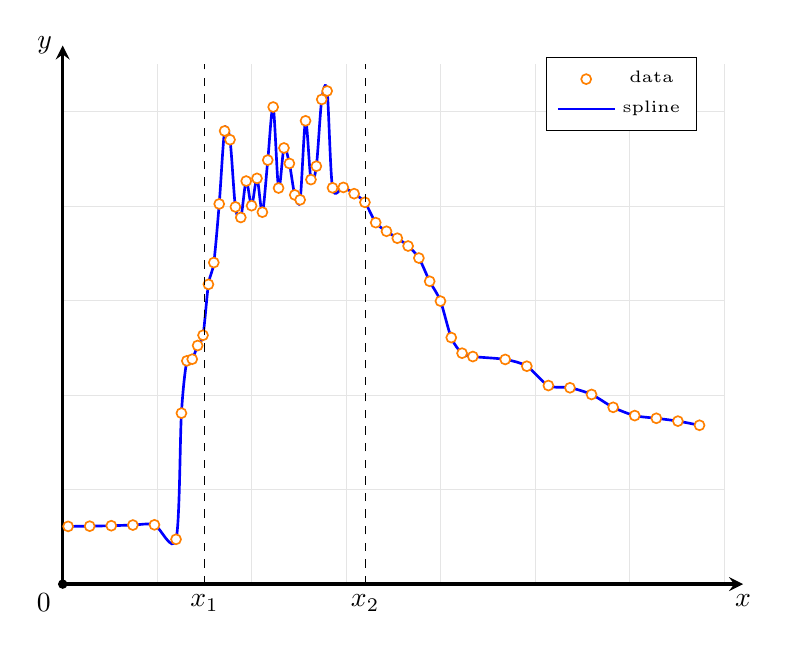
\begin{tikzpicture}[
	scale=1.2,
	axis/.style={
		-stealth,
		very thick
	}
]
% Gitter
\draw[gray!20] (0,0) grid (7,5.5);

% Achsen
\draw[axis] (0,0) -- (0,5.7) node[left]{$\boldsymbol{y}$};
\draw[axis] (0,0) -- (7.2,0) node[below]{$\boldsymbol{x}$};
\fill[black] (0,0) circle[radius=0.05];
\node at(-0.2,-0.2){$\boldsymbol{0}$};
	\begin{axis}[axis lines=none, xmin=40, xmax=160, mark size=1.5pt, legend style={font=\tiny}]
	%\pgfplotstableread{data/data.txt}
	%\datatable
	\addplot [mark=*,
			  only marks,
			  mark options={line width=0.5pt, color=orange,fill=white}]
                coordinates{
                (41,0.06030273)(45,0.10046387)(49,0.18066406)(53,0.30114746)(57,0.34130859)(61,-2.25805664)(62,20.40356445)(63,29.79736328)(64,30.09851074)(65,32.54736328)(66,34.39404297)(67,43.53698730)(68,47.45104980)(69,57.97900391)(70,71.09619141)(71,69.52062988)(72,57.44702148)(73,55.55017090)(74,62.09375000)(75,57.66784668)(76,62.57556152)(77,56.50366211)(78,65.85742188)(79,75.39172363)(80,60.83923340)(81,68.03527832)(82,65.25524902)(83,59.60485840)(84,58.72167969)(85,72.91284180)(86,62.35473633)(87,64.76342773)(88,76.75659180)(89,78.27209473)(90,60.87939453)(92,60.94970703)(94,59.82568359)(96,58.27001953)(98,54.62695312)(100,53.07128906)(102,51.82678223)(104,50.42175293)(106,48.26391602)(108,44.08886719)(110,40.52612305)(112,33.97241211)(114,31.17236328)(116,30.57019043)(122,30.04833984)(126,28.83398438)(130,25.36145020)(134,24.95996094)(138,23.75561523)(142,21.44738770)(146,19.96203613)(150,19.48022461)(154,18.96838379)(158,18.22570801)
                };
                \addlegendentry{data}
    
    \addplot [smooth,
			  color=blue,
			  thick]
                coordinates{
                (41,0.06030273)(45,0.10046387)(49,0.18066406)(53,0.30114746)(57,0.34130859)(61,-2.25805664)(62,20.40356445)(63,29.79736328)(64,30.09851074)(65,32.54736328)(66,34.39404297)(67,43.53698730)(68,47.45104980)(69,57.97900391)(70,71.09619141)(71,69.52062988)(72,57.44702148)(73,55.55017090)(74,62.09375000)(75,57.66784668)(76,62.57556152)(77,56.50366211)(78,65.85742188)(79,75.39172363)(80,60.83923340)(81,68.03527832)(82,65.25524902)(83,59.60485840)(84,58.72167969)(85,72.91284180)(86,62.35473633)(87,64.76342773)(88,76.75659180)(89,78.27209473)(90,60.87939453)(92,60.94970703)(94,59.82568359)(96,58.27001953)(98,54.62695312)(100,53.07128906)(102,51.82678223)(104,50.42175293)(106,48.26391602)(108,44.08886719)(110,40.52612305)(112,33.97241211)(114,31.17236328)(116,30.57019043)(122,30.04833984)(126,28.83398438)(130,25.36145020)(134,24.95996094)(138,23.75561523)(142,21.44738770)(146,19.96203613)(150,19.48022461)(154,18.96838379)(158,18.22570801)
                };
                \addlegendentry{spline}
	\end{axis}
	
	\node at(1.5,-0.2){$x_1$};
	\node at(3.2,-0.2){$x_2$};
	\draw[dashed] (1.5,0) -- (1.5,5.5);  
	\draw[dashed] (3.2,0) -- (3.2,5.5);  


\end{tikzpicture}
\caption[Graphische Darstellung der nichtparametrischen Regression]{Graphische Darstellung der nichtparametrischen Regression\protect\footnotemark}
\label{pr}
\end{figure}
\footnotetext{Abb. in Anlehnung an \textit{Günther}, Mathematische Modellbildung und Simulation, 2014, S. 92.}
\textit{\glqq Splinefunktionen gehören zu den wichtigsten und verbreitetsten Regressionsmethoden und werden quer durch alle Disziplinen z.B. in Betriebswirtschaft, Informatik, Bildverarbeitung, Medizin, Maschinen usw. angewendet.\grqq}\seFootcite{}{S.93}{Gunther.2014} 

\enlargethispage{\baselineskip}Der Gedanke der \textit{smoothing splines}\footnote{Die englische Übersetzung bedeutet so viel wie \textit{glättende Verzahnung}} ist, den Bereich der $x$-Werte durch ein feines Gitter so zu unterteilen, sodass sich die angrenzenden Intervalle durch glatt miteinander verbundene Polynomfunktionen niedrigen Grades (oftmals kubisches Polynom) approximieren lassen.\seFootcite{Vgl.}{S. 510}{Fahrmeir.2007} In \vref{splineZoom} ist dazu die Punktewolke aus \vref{pr} im Wertebereich zwischen $x_1$ und $x_2$ genauer dargestellt, um das Resultat dieses Verfahrens besser betrachten zu können. Legt man das Augenmerk ausschließlich auf den Intervallbereich $I_i$, so lässt sich dieser Bereich durch ein kubisches Polynom ausdrücken. Werden all diese Intervalle als eigene Funktionen definiert und stückweise an den \glqq Knotenpunkten\grqq~(Übergang zwischen den einzelnen Intervallen) stetig und differenziert aneinander gesetzt, erhält man die gesuchte Regressionsfunktion $\hat{f}(x)$.\seFootcite{Vgl.}{S. 510}{Fahrmeir.2007}
\end{itemize}
\begin{figure}[H]
\centering
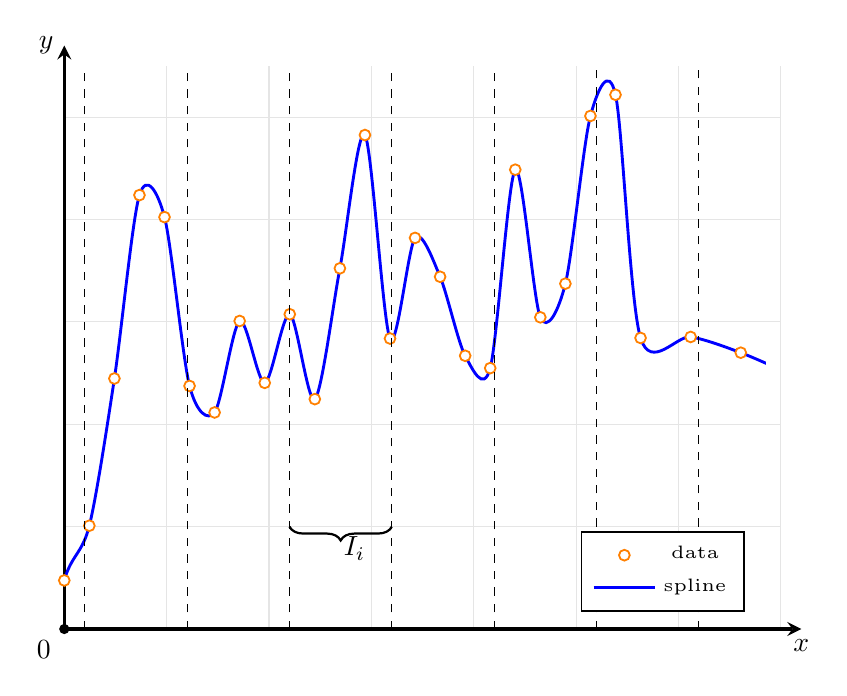
\begin{tikzpicture}[
	scale=1.3,
	axis/.style={
		-stealth,
		very thick
	}
]
% Gitter
\draw[gray!20] (0,0) grid (7,5.5);

% Achsen
\draw[axis] (0,0) -- (0,5.7) node[left]{$\boldsymbol{y}$};
\draw[axis] (0,0) -- (7.2,0) node[below]{$\boldsymbol{x}$};
\fill[black] (0,0) circle[radius=0.05];
\node at(-0.2,-0.2){$\boldsymbol{0}$};

	% Geschweifte Klammer
\draw[
	thick,
	black,
	decorate,
	decoration = {
		brace,
		amplitude = 5pt
	}
] (3.2,1) -- (2.2,1)
	node[
		midway,
		below,
		xshift = 5pt
] {$\boldsymbol{\small I_i}$};


	\begin{axis}[axis lines=none, xmin=67, xmax=95, mark size=1.5pt, legend style={font=\tiny}, legend pos=south east]
	%\pgfplotstableread{data/data.txt}
	%\datatable
	\addplot [mark=*,
			  only marks,
			  mark options={line width=0.5pt, color=orange,fill=white}]
                coordinates{(65,32.54736328)(66,34.39404297)(67,43.53698730)(68,47.45104980)(69,57.97900391)(70,71.09619141)(71,69.52062988)(72,57.44702148)(73,55.55017090)(74,62.09375000)(75,57.66784668)(76,62.57556152)(77,56.50366211)(78,65.85742188)(79,75.39172363)(80,60.83923340)(81,68.03527832)(82,65.25524902)(83,59.60485840)(84,58.72167969)(85,72.91284180)(86,62.35473633)(87,64.76342773)(88,76.75659180)(89,78.27209473)(90,60.87939453)(92,60.94970703)(94,59.82568359)(96,58.27001953)
                };
                \addlegendentry{data}
    
    \addplot [smooth,
			  color=blue,
			  thick]
                coordinates{(65,32.54736328)(66,34.39404297)(67,43.53698730)(68,47.45104980)(69,57.97900391)(70,71.09619141)(71,69.52062988)(72,57.44702148)(73,55.55017090)(74,62.09375000)(75,57.66784668)(76,62.57556152)(77,56.50366211)(78,65.85742188)(79,75.39172363)(80,60.83923340)(81,68.03527832)(82,65.25524902)(83,59.60485840)(84,58.72167969)(85,72.91284180)(86,62.35473633)(87,64.76342773)(88,76.75659180)(89,78.27209473)(90,60.87939453)(92,60.94970703)(94,59.82568359)(96,58.27001953)
                };
                \addlegendentry{spline}
	\end{axis}
	\draw[dashed] (0.2,0) -- (0.2,5.5);  
	\draw[dashed] (1.2,0) -- (1.2,5.5); 
	\draw[dashed] (2.2,0) -- (2.2,5.5);  
	\draw[dashed] (3.2,0) -- (3.2,5.5); 
	\draw[dashed] (4.2,0) -- (4.2,5.5); 
	\draw[dashed] (5.2,0) -- (5.2,0.19);  
	\draw[dashed] (6.2,0) -- (6.2,0.19);  
	\draw[dashed] (5.2,1) -- (5.2,5.5);  
	\draw[dashed] (6.2,1) -- (6.2,5.5);  
	
	%\draw[<-,->] (2.2,1) -- (3.2,1) node[below, midway] {\small $I_i$};
	


\end{tikzpicture}
\caption[Anwendung der \textit{Spline}-Regression]{Anwendung der \textit{Spline}-Regression\protect\footnotemark}
\label{splineZoom}
\end{figure}
\footnotetext{Eigene Darstellung: Vergrößerung der Punktewolke aus \vref{pr} im Wertebereich $x_1$ bis $x_2$}



\paragraph{Bewertung} Wie in der Einleitung dieses Kapitels beschrieben, wird die Wahrscheinlichkeit eines Torerfolges durch mehrere Faktoren, wie beispielsweise den Koordinaten des Schusses, beeinflusst, wodurch die \textit{lineare Regression} für die Modellierung ausgeschlossen werden kann, da die Zielvariable in der vorliegenden Problemstellung von mindestens zwei unabhängigen Variablen abhängt. In einem multiplen Regressionsmodell können mehrere unabhängige Variablen behandelt werden, wobei auch hier von vornherein eine parametrische Spezifikation der Funktion angegeben werden müsste. Eine erste mögliche Vorstellung in Bezug dazu wäre hierzu die Funktion $\hat{f}(x_1,x_2) = \alpha_0 e^{-x_1} \cdot \alpha_1\sin(\alpha_2 \cdot (\pi x_2 - \alpha_3))$, die in \vref{vermutung} abgebildet ist. 
\begin{figure}[H]
\centering
\def\axislength{.2}
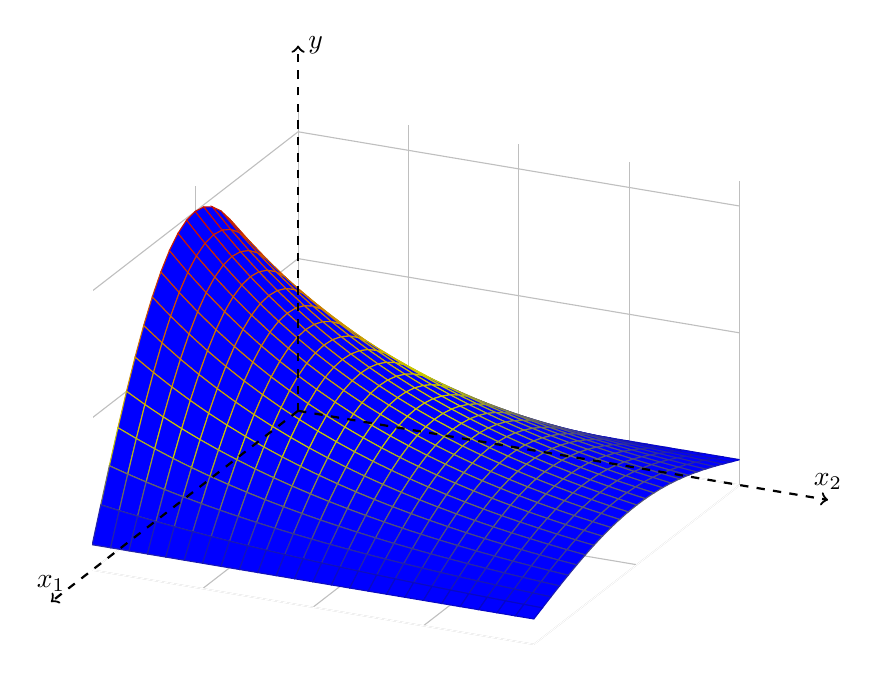
\begin{tikzpicture}
\pgfplotsset{
    axis line style={white},
  }
  \begin{axis}[scale=1.2,ticks=none, grid=major, legend style={at={(1.1,1.1)},anchor=north west} ]
    \coordinate (O) at (rel axis cs:0,1,0);
    \coordinate (x) at (rel axis cs:0,-\axislength,0);
    \coordinate (y) at (rel axis cs:1+\axislength,1,0);
    \coordinate (z) at (rel axis cs:0,1,1+\axislength);
    \addplot3[surf,shader=faceted,
			samples=25,domain=0:2,y domain=0:1, color=blue] {exp(-x) * sin(pi*deg(y))};
  \end{axis}
  \draw[thick,dashed,->] (O) -- (x) node[above] {$\boldsymbol{x_1}$};
  \draw[thick,dashed,->] (O) -- (y) node[above] {$\boldsymbol{x_2}$};
  \draw[thick,dashed,->] (O) -- (z) node[right] {$\boldsymbol{y}$};

  
\end{tikzpicture}
\caption[Erste Vorstellung der Funktion]{Erste Vorstellung der Funktion\protect\footnotemark}
\label{vermutung}
\end{figure}
\footnotetext{Eigene Darstellung in Bezug auf die Koordinaten des Schusses.}

Die Parameter $x_1$ (=Breite des Spielfeldes) und $x_2$ (=Länge des Spielfeldes) geben hierbei die Koordinaten an, von dem geschossen wurde, wobei das gegnerische Tor auf der $x_1$-Achse -- also bei $x_2=0$ -- mittig platziert ist. Die Vermutung ist, dass die Wahrscheinlichkeit $y$ mit zunehmender Nähe zum Tor steigt, wodurch sich die Fläche in Richtung Tor stetig erhöht und eine Art \glqq Gipfel\grqq~ entsteht. Bereits bei der Betrachtung dieser Vermutung ist zu erkennen, dass eine \glqq herkömmliche\grqq~mathematische Funktion das Ergebnis zu einer sehr verfälschenden Anpassung führt. Wenn beispielsweise ein Schuss auf der Höhe der Grundlinie seitlich des Tores abgegeben wurde, dann ist aufgrund des Winkels ein Torerfolg fast unmöglich und die Wahrscheinlichkeit somit falsch repräsentiert. Folglich ist es sinnvoll, \textit{nichtparametrische Regressionsfunktionen} in Form von \textit{Splines} zu verwenden, um eine exakte Anpassung der Funktion an die vorliegenden Daten zu erreichen. Eine detaillierte Gegenüberstellung der multiplen und nichtparametrischen Regression wird innerhalb der Umsetzung in \vref{mdf} aufgezeigt.

%%%%%%%%%%%%% BESTIMMTHEITSMASS %%%%%%%%%%%%%%%%%%
\subsubsection{Bestimmtheitsmaß}
\label{bhm}
Um die Qualität der Anpassung des Modells an die Daten zu überprüfen, stellt der graphische Vergleich zwischen Modell und Daten die simpelste Möglichkeit dar. Betrachtet man nochmals die Sinus-Funktion aus \vref{nlr}, ist zu erkennen, dass das Modell sehr gut an die Daten angepasst wurde.\seFootcite{Vgl.}{S.71}{Gunther.2014} Für eine exakte Modellierung ist jedoch das Bestimmtheitsmaß $R^2$ notwendig, welches den \textit{goodness of fit} (\textit{dt. Anpassungsgüte}) misst.\seFootcite{Vgl.}{S. 51}{Studenmund.2014} Die Qualität des Modells wird dabei auf einer Skala von 0 und 1 dargestellt, wobei ein sehr hoher Wert für eine gute Anpassung und ein niedriger Wert für eine schlechte Anpassung des Modells an die Daten spricht. Diese Skala dient dazu, verschiedene Regressionsmodelle miteinander zu vergleichen.\seFootcite{Vgl.}{S.71}{Gunther.2014} Das Bestimmtheitsmaß $R^2$ misst dabei, zu welchem prozentualen Anteil die Abweichung der gemessenen abhängigen Variablen durch die unabhängigen Variablen des Modells erklärt wird und ist formal wie folgt definiert:\seFootcite{Vgl.}{S.118}{Daroczi.2015}\seFootcite{Vgl.}{S.72}{Gunther.2014}\seFootcite{Vgl.}{S. 51}{Studenmund.2014}

\begin{equation}
R^2 = 1 - \frac{\sum\limits_{i=1}^n (y_i - \hat{y}_i)^2}{\sum\limits_{i=1}^n (y_i - \overline{y})^2}= \frac{RSS}{TSS}
\label{r2}
\end{equation}

Wie in \vref{r2} zu erkennen ist, kann das $R^2$ auch als Verhältnis von \gls{rss} zu der \gls{tss}, also der erklärten Variation zur gesamten Abweichungsqudratsumme, dargestellt werden.\seFootcite{Vgl.}{S. 48}{Studenmund.2014}\seFootcite{Vgl.}{S.119}{Daroczi.2015} Die Hinzunahme von weiteren erklärenden $x$-Variablen führt im schlechtesten Fall dazu, dass das Bestimmtheitsmaß gleich bleibt, unabhängig davon, ob die zusätzlichen Variablen die Qualität des Modells verbessern oder nicht. Man spricht dabei von einer \textit{Überparametrisierung} des Modells.\seFootcite{Vgl.}{S. 160}{Cleff.2008} Um diesen Fall zu vermeiden, verwendet man in der Praxis das \textit{korrigierte Bestimmtheitsmaß} $\overline{R}^2$ (\textit{engl.: adjusted $R^2$}), welches die Hinzunahme von Variablen mit geringer Erklärungskraft \glqq bestraft\grqq~(die Qualität der Anpassung sinkt).\seFootcite{Vgl.}{S. 161}{Cleff.2008} Die Hinzunahme einer zusätzlichen Variable in die Modellierung sollte nur dann in Erwägung gezogen werden, wenn der dadurch gewonnene Erklärungswert für das Modell größer als der \glqq Bestrafungsabschlag\grqq~des korrigierten Bestimmtheitsmaßes ist. Das korrigierte $\overline{R}^2$ kann daher zum Vergleich von Regressionsmodellen mit einer unterschiedlicher Anzahl von unabhängigen Variablen herangezogen werden, um die Anpassungsgüte des Modells an die Daten zu messen.\seFootcite{Vgl.}{S. 56}{Studenmund.2014} Die ursprüngliche Interpretation von $R^2$ geht jedoch durch die \glqq Bestrafung\grqq~der Hinzunahme weiterer Parameter weites gehend verloren, sodass beide Bestimmtsheitsmaße für eine Bewertung herangezogen werden sollten.\seFootcite{Vgl.}{S. 161}{Cleff.2008} 

In diesem Kontext spricht man in der Fachsprache auch von \textbf{Overfitting}, einer Überanpassung des Modells durch Hinzunahme irrelevanter Variablen, die zu einer unnötigen Steigerung der Komplexität des Modelles führen. Das Modell scheint dabei für die vorliegenden Daten exakt zu passen, scheitert jedoch bei der Prognose von noch ungesehenen Daten. \textbf{Underfitting} ist die gegenteilige Bezeichnung und beschreibt ein zu simplel gewähltes Modell, welches zu wenig relevante Regressoren enthält und folglich eine geringe Anpassung der Funktion an die Daten aufweist.\seFootcite{Vgl.}{S. 470}{Cios.2007} 


